\section{System}\label{sec:System}
This chapter describes the contour searching method and different approaches to estimate the light direction of an object in detail. In the beginning, the contours of an object of interest are generated in the application to get all pixel coordinates along an adequate contour patch. Followed by the actual computations to ascertain the light direction of an infinitive light source that shines on the object belonging to the contour patch. All necessary steps to calculate the light direction can be done and understood in the GUI described in section~\ref{sec:GUI}.

\subsection{Contours}\label{sec:contours}
To estimate the light direction of an object in a digital image, it is firstly necessary to locate the object of interest and get its shape information. All information are described by the contour, which is forced to be perfectly even to guarantee a successful light direction estimation. The most important required information are all pixel coordinates along the outer bound of the object in an ordered way.

Beside a correctly localisation, an application with a good usability is preferred as well. An pre implemented interactive segmentation \cite{website:LiveWire} was integrated into the application to generate the affordable contours with manual constraints that are defined by the user. This method is called \textit{Live-Wire}~\cite{BARRETT1997331} and based on a maximum flow problem. However, several test showed that this extension calculates noisy and fault contours as well as it lacks of robust control options for the user. The main problem was that the generated contour seems to follow the valley between two edges of an RGB image and snap to the most significant edge in a wide neighbourhood. Even more, constraints set by the user did not result in adequate and useful contours. 

Due to the fact that those results were unusable, the team decided to extract the contours from perfectly even mask images of the objects of interest like shown in Figure \ref{fig:batch1mask}. These images are prepared manually in \textit{Adobe Photoshop CS 6} with the pen tool that offers perfectly round and even Bezier curves. All created masks are shrink about almost two pixels to ensure that only pixel information of the actual object are used for further proceedings and none from the background. 

If the file name of a mask image is the same as the one belonging to the selected RGB image with the extension \texttt{\_mask.jpg}, it will be loaded automatically into the application at the same time when the belonging RGB image is opened (compare Section~\ref{sec:GUI}). This mask data will be used for all further contour calculations.

\begin{figure} [H]
	\center 
	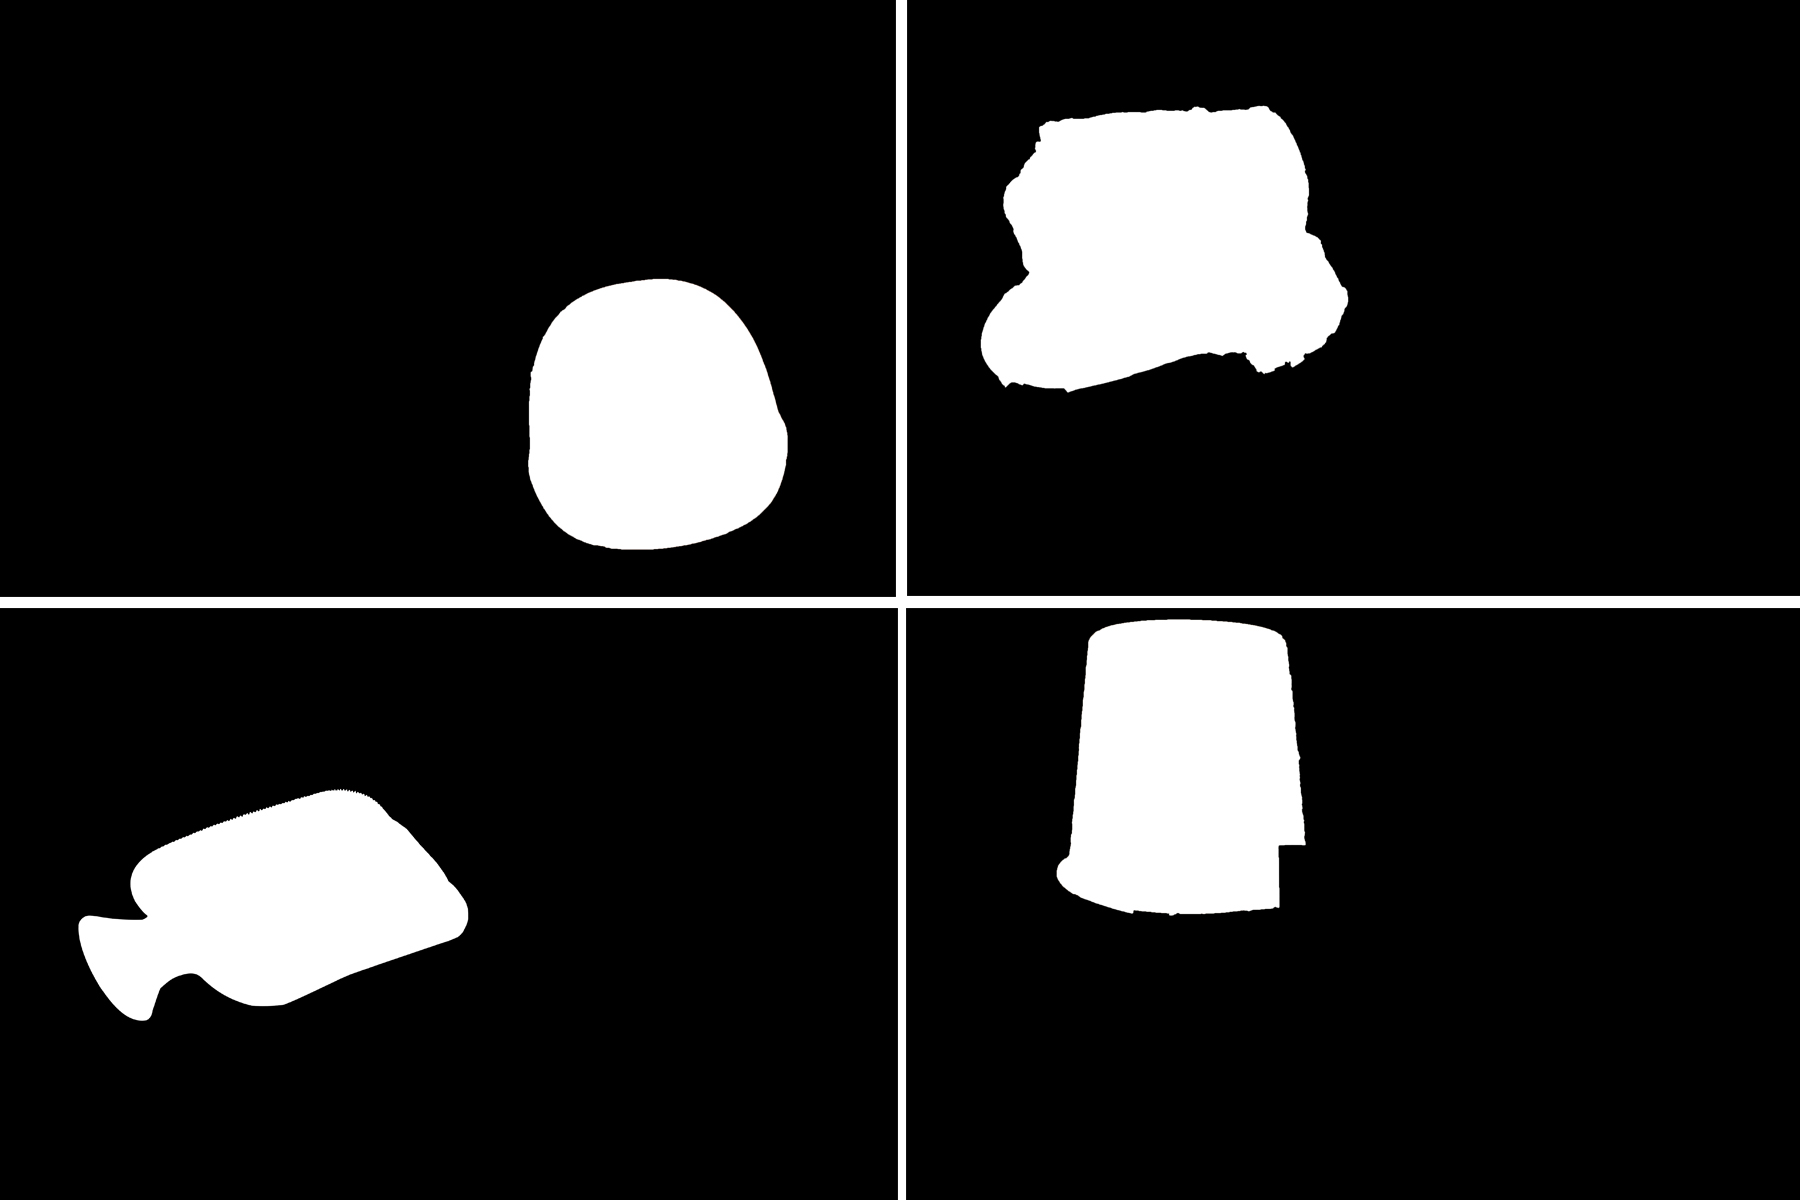
\includegraphics[width=12cm]{Images/batch1_mask.jpg}			
	\caption[Bildunterschrift]{Manual created mask images of the first batch.}
	\label{fig:batch1mask}
\end{figure}

\subsubsection{Calculate Contours}\label{sec:findContours}
Several \textit{OpenCV} (compare Section \ref{sec:opencv}) functions are used to compute all required pixel coordinates along the outer object boundary. In the beginning a common erosion filter with a filter size of three is applied to the mask image to eliminate small outliers and in order to shrink the mask to ensure that it is not located directly or outside the object boundary. In the next step, a Canny filter with a filter size of five is used to extract the edges. Then the \textit{OpenCV} function \texttt{findContours()} calculates the vector representations of the binary canny image with the border following algorithm of Suzuki et Al.~\cite{SUZUKI198532}. All results are not optimized by any approximations because otherwise important coordinate data will be lost. The resulting contours will be printed into the preview of the GUI (compare Setcion \ref{sec:GUI}) to allow the user a selection of a suitable sub-contour to feed the light direction estimation.

\subsection{Generate Subcontours}\label{sec:subcontours}
As mentioned, the user is forced to select an adequate part of the contour to contain the further calculations. He can do so in the GUI with a simple rectangle selection in the preview. This selection can be renewed, if affordable, and saved. After the storage of all contour points within the rectangle, they are stored and sorted in a so called  sub-contour. At this point, the sort is needed because all contour points are stored like a ring buffer that starts at the highest point and then follows counter clock wise the boundary. Thus, it has to be reordered to ensure an open and gapless sub-contour, if the selection includes the top of the complete contour.

After this process, we have a sub-contour that includes all important edge points along the boundary but it still lacks of all pixel coordinates along this part of the boundary.
This circumstance can be solved by making a binary image and print the required sub-contour into it with a line thickness of one pixel. Then a \textit{OpenCV} \texttt{LineIterator} is applied to this image. It is treated as versatile implementation of the Bresenham algorithm~\cite{5388473} and allows the notice and storage of every required coordinate. Now, these coordinates can be used for the following approaches of the light direction estimation in a single digital image.


\subsection{Illumination Model}\label{sec:lightingmodel}
To understand the following approaches (compare Section~\ref{sec:approaches}), it is useful to give a short introduction to the definition of an illumination model. One of the most acknowledged illumination model is the Blinn model~\cite{Blinn:1977}(compare Equation\ref{equ:Blinn}) which defines a basic illumination in a three dimensional space. In this model is $\vec{n}$ the surface normal, $\vec{l}$ the light direction vector and $\vec{h}$ is the direction of the maximum highlights. All $p$ variables that are related to the proportions of each reflection type which are part of the sum and $s$ is the amount of the specular reflection. This illumination is finally a simple sum of the ambient $a$, diffuse $d$ and specular $sp$ light parts. 
\begin{equation}
\label{equ:Blinn}
I(x,y,z) = (\vec{n}\cdot \vec{l})*p_d + (\vec{n}\cdot\vec{h})^s*p_s + p_a = d + sp + a
\end{equation} 

Due to the high number of unknown variables and vectors, the Blinn model is too complex to calculate the 3-dimensional vector $\vec{l}$ with standard approaches like the least square method. Hence, some assumptions to simplify the mode had to be made~\cite{Johnson}. The first assumption is to state the current surface reflects light isotropically. This surface has a constant reflectance value $r$ and is illuminated by a faraway infinitive light source. Finally, the angle between $\vec{n}$ and  $\vec{l}$ is in the range of $0^\circ $ and $90^\circ$. All previous assumptions lead to the simplified light model of equation \ref{equ:simpleLightmodel}.

\begin{equation}
\label{equ:simpleLightmodel}
I(x,y,z) = r(\vec{n}\cdot \vec{l}) + a
\end{equation} 

\subsection{Different Approaches}\label{sec:approaches}
Three different approaches were tried out because a reliable solution could not be found. All approaches are based on the paper of Johnson and Farid \cite{Johnson}. 
Two of this approaches remained unchanged (compare Section~\ref{sec:appOne} and \ref{sec:appTwo}) but the last approach takes the assumptions of Johnson and Farid and expand them (compare Section~\ref{sec:appThree}). \\
In the following sections, it has to be noted, that we do not have a three dimensional space like almost all other light direction estimations, which are based on images. All realised approaches of Johnson are based on a infinite light source in a two dimensional image space. \\
The basic idea of the approach is a simplified light model that is described in Section~\ref{equ:Blinn}. To differentiate the 2D case all parameters are written in upper letters. In 2D Equation~\ref{equ:simpleLightmodel} is referred to as follows:

\begin{equation}
\label{equ:General}
I(x,y) = R(\vec{N}(x,y)\cdot \vec{L}) + A
\end{equation}

To standardise the explanations in the following sections a list of necessary variables is introduced: 
\begin{itemize}
\item $\vec{L} \in \mathbb{R}^2$: vector, which points in the direction of the light source 
\item $\vec{N}(x,y)\in \mathbb{R}^2$: surface normal at the point (x,y) 
\item $I(x,y)$: intensity at the point (x,y)
\item $A$: constant ambient light term
\item $R$: constant reflectance value
\end{itemize}
All equations in this section, as well as its subsections, are taken from \cite{Johnson}. \\
For the second and the third approach, the light vectors are summed up in patches of a size of four pixel. 

\subsubsection{1. Approach: One Lightvector}\label{sec:appOne}

The first approach tries to simplify the two dimensional case by solving Equation \ref{equ:firstApp} and getting one final light vector per sub-contour plus the ambient light term. The Matrix $M$, which contains the surface normals, can be found in Johnsons and Farids paper \cite{Johnson} in Equation (6) and $p$ denotes the number of points on a contour with the same assumed reflectance. All other variables are explained in Section~\ref{sec:approaches}. Thereby, the reflectance along the entire contour is thought as constantly. 

\begin{equation}
\label{equ:firstApp}
E(\vec{L} , A) = 
\left\vert \left\vert 
M
\begin{pmatrix}
L_{x} \\
L_{y} \\
A \\
\end{pmatrix} -
\begin{pmatrix}
I(x_{1} , y_{1}) \\
I(x_{2} , y_{2}) \\
\vdots \\
I(x_{p} , y_{p}) \\
\end{pmatrix}
 \right\vert\right\vert^{2}
 = \left\vert \left\vert  M\vec{v}-\vec{b}  \right\vert\right\vert^{2}
\end{equation}

This options can be activated in our script \texttt{mainwindow.cpp} by setting the variable \texttt{usePatches} to \texttt{false}. Equation~\ref{equ:firstApp} is then solved by using the \textit{Singular Value Decomposition}. The resulting light vector $\vec{L}$ is drawn into the test image to visualize the result.  

\subsubsection{2. Approach: Averaging Lightvectors}\label{sec:appTwo}

For the second approach, it is not only assumed that the light source is infinite, but also that the reflection, created by it, is constant within each surface patch. A more detailed description of this approach can be found in section 2.2.1 in the paper of Johnson and Farid \cite{Johnson}.\\
It is assumed, that a minimization problem according to Equation~\ref{equ:secondApp} needs to be solved. The related Matrix $M$ can be found in \cite{Johnson} in Equation (8). \\

\begin{equation}
\label{equ:secondApp}
E_{1}(\vec{L}^{\,1} , ... , \vec{L}^{\,n} , A) = 
\left\vert \left\vert 
M
\begin{pmatrix}
L^{1}_{x} \\
L^{1}_{y} \\
\vdots  \\
L^{n}_{x} \\
L^{n}_{y} \\
A \\
\end{pmatrix} -
\begin{pmatrix}
I(x^{1}_{1} , y^{1}_{1}) \\
\vdots  \\
I(x^{1}_{p} , y^{1}_{p}) \\
\vdots  \\
I(x^{n}_{1} , y^{n}_{1}) \\
\vdots  \\
I(x^{n}_{p} , y^{n}_{p}) \\
\end{pmatrix}
 \right\vert\right\vert^{2}
 = \left\vert \left\vert  M\vec{v}-\vec{b}  \right\vert\right\vert^{2}
\end{equation}
This options can be activated in our script \texttt{mainwindow.cpp} by setting \texttt{usePatches} to \texttt{true} and \texttt{useHighestIntensity} to \texttt{false}.
As stated in Section~\ref{sec:appOne}, Equation~\ref{equ:secondApp} is solved using \textit{Singular Value Decomposition} as well. This leads to calculating one light vector per patch. To get the final vector $\vec{L}$ all these light vectors are averaged.


\subsubsection{3. Approach: Lightvector with maximum Intensity}\label{sec:appThree}

This last approach uses the same basic idea as the second one described in section \ref{equ:secondApp}. It is also based on dividing the surface normals $\vec{N}$ into patches and solving Equation~\ref{equ:secondApp} using \textit{Singular Value Decomposition}. Afterwards, there is no averaging done but the vector $\vec{L}$ belonging to the patch with the maximum intensity is taken as the final light vector. \\
This idea is not described in the paper of Johnson and Farid~\cite{Johnson}. It was a try to make the results of the \textit{Interactive Lighting Detector} more trustworthy and reproducible. \\
This options can be activated in our script \texttt{mainwindow.cpp} by setting \texttt{usePatches} to \texttt{true} and \texttt{useHighestIntensity} to \texttt{true}.


\subsection{Graphic User Interface} \label{sec:GUI}

As the \textit{Interactive Lighting Detector} is implemented as an half-automatic application, a GUI is needed to give the user the opportunity to make decisions. The GUI leads the user from loading an image to the final results. Here, an expiry is given. For reasons of space all corresponding screenshots can be found in the attachment (compare Section~\ref{sec:Attachment}).  
\begin{itemize}
\item \textbf{loading an image:} If the user presses the button \textit{Load Image}, he can chose an image from his hard disk drive, which has the file format JPEG or Tiff (compare figure~\ref{fig:Gui01}). In addition, the mask image is then loaded in the background as described in Section~\ref{sec:contours}.
\item \textbf{contour detection:} Once an image is loaded, the \textit{Run Contour Detection}-button gets visible. After clicking on it the contour is drawn onto the displayed image.
\item \textbf{sub contour:} As the algorithm does not need a closed contour, the user can select a subcontour by pressing the \textit{Select Part of Contour}-button and drawing a rectangle, including the part of the contour (marked in green) he wants to select (compare figure~\ref{fig:Gui02}). If he is dissatisfied with his selection he can renew it by pressing the \textit{Delete Selection}. Otherwise he can apply the selection by pressing the \textit{Save Selection}. 
\item \textbf{calculating normals:} By clicking the \textit{Show Normals}-button the surface normals for the subcontour are determined and drawn in red (compare figure~\ref{fig:Gui03}).
\item \textbf{calculating lightvectors:} The last step is to calculate the lightvectors by pressing the \textit{Show Lightvectors}-button. The final lightvector is then drawn in blue. If it is chosen to calculate the light vectors for every single patch (compare section \ref{sec:approaches}), than all other light vectors are drawn in white (compare figure~\ref{fig:Gui04}). 
\end{itemize}

To simplify the expiry the GUI can be refreshed by pressing the \textit{Restart}-button. In addition to that the application can be closed at any time \textcolor{red}{Wo?}. 


\newpage